\documentclass[a4paper]{article}
\usepackage{listings}
\usepackage[isolatin]{inputenc}
\usepackage{makeidx,times}
\usepackage{fancyhdr}
\usepackage{graphicx}
\usepackage{float}
\usepackage{alltt}
%%\usepackage{doxygen}
\usepackage[pdftex,
            pagebackref=true,
            colorlinks=true,
            linkcolor=blue
           ]{hyperref}
           
\makeindex
\lstset{tabsize=1,language=C++,basicstyle=\small}
\author{J. Andreas B{\ae}rentzen}
\title{Introduction to GEL\\\vspace{0.25cm} \normalsize
\textit{An informal introduction to the GEL library with many examples of usage}.}
\setcounter{tocdepth}{2}
\begin{document}
\maketitle
\tableofcontents
\newpage
%
%
\section{Introduction}
%
%
\sloppy
GEL is an abbreviation of GEometry and Linear algebra. GEL is a C++ library with tools for manipulating digital representations of geometry such as polygonal meshes, triangle meshes, point clouds, and voxel grids. Since linear algebra tools are invariably needed for this, GEL also contains tools for linear algebra. Finally, GEL contains tools for drawing geometry using OpenGL and various utilities.

This document pertains to the version of GEL which is distributed on CampusNet for 02585. This version of GEL comes with project files for Visual Studio 9 and XCode and examples relevant for the course are included in the distribution.

GEL is not documented as well as we would like, but a fair amount of Doxygen documentation is provided for those parts of GEL which are used a lot. You will find the reference manual at \href{http://www2.imm.dtu.dk/courses/02585/GELref/index.html}{http://www2.imm.dtu.dk/courses/02585/GELref/index.html}

Please use it. Autogenerated documentation is not eminently readable, but it is much better than no documentation and it should be relatively complete for the parts of GEL needed in the course. 

The goal of \textit{this} document is to provide more detail and to help people getting started. In particular, this document focuses on functionality in the CGLA and HMesh namespaces, but we shall also take a look at some other parts of GEL. Unfortunately, it is rather difficult to be complete: There is functionality in GEL not covered here. Consequently, if you are looking for something particular, we \textbf{entreat } you to look at the reference linked to above
\subsection{Overview of GEL}

GEL contains many tools for geometry processing and a number of data structures. Perhaps the most important is the \texttt{Manifold} class which resides in the \texttt{HMesh} namespace. A \texttt{Manifold} is a halfedge based representation of a polygonal mesh. There is also a simpler triangle mesh data structure, \texttt{TriMesh}, based on an indexed face set. There are several voxel grid data structures, a fairly efficient k-D tree for storing points, bounding box hierarchies etc.

A number of algorithms exist for manipulating these representations of geometric data. For instance, \texttt{Manifold} has a function for mesh simplification, several functions for smoothing (including anisotropic), mesh optimization, and mesh clean up.
Another strong point of GEL is the fact that it contains good support for converting between representations; especially between meshes and voxel grids. There are several tools for polygonizing isosurfaces and also converting meshes to distance fields.  The tools pertaining to the Manifold data structure are in the \texttt{HMesh} namespace. The other geometry related tools are in the \texttt{Geometry} namespace.

There are two packages for linear algebra: \texttt{CGLA} is strictly for small vectors and matrices (dimensions 2,3, and 4). \texttt{LinAlg} is a Lapack wrapper for slightly larger problems. At this point, it is fairly simple but includes a number of functions for solving linear systems, factoring matrices and finding eigensolutions for symmetric matrices.

\texttt{GLGraphics} contains facilities for drawing entities from other parts of GEL via OpenGL. Especially \texttt{TriMesh} and Manifold have good support. For instance, there is a nice wireframe drawing class. There are also two virtual trackballs for interactive programs and some tools for viewing in interactive programs and SOIL a small open source library for image loading by Jonathan Dummer.

Finally there are some utilities in \texttt{Util}: Getting command line arguments, hash table classes, a 2D grid class, a resource manager, an XML parser by Jeppe Frisvad and other tools.
%
%
\section{CGLA}
%
%
\texttt{CGLA} is a set of numerical C++ vector and matrix classes and class
templates designed with computer graphics in mind. \texttt{CGLA} stands for
``Computer Graphics Linear Algebra''. Let us get right down to the obvious question: Why create another
linear algebra package?
Well, \texttt{CGLA} evolved from a few matrix and vector classes because I
didn't have anything better. Also, I created \texttt{CGLA} to experiment with
some template programming techniques. This led to the most important
feature of \texttt{CGLA}, namely the fact that all vector types are derived
from the same template. 

This makes it easy to ensure identical semantics: Since all vectors
have inherited, say, the * operator from a common ancestor, it works
the same for all of them.

It is important to note that \texttt{CGLA} was designed for Computer Graphics 
(not numerical computations) and this had a number of
implications. Since, in computer graphics we mainly need small vectors
of dimension 2,3, or 4 \texttt{CGLA} was designed for vectors of low
dimensionality. Moreover, the amount of memory allocated for a vector
is decided by its type at compile time. \texttt{CGLA} does not use dynamic
memory. \texttt{CGLA} also does not use virtual functions, and most functions
are inline. These features all help making \texttt{CGLA} relatively fast. 

Of course, other libraries of vector templates for computer graphics
exist, but to my knowledge none where the fundamental templates are
parametrized w.r.t. dimension as well as type. In other words, we have
a template (\texttt{ArithVec}) that gets both type
(e.g. \texttt{float}) and dimension 
(e.g. 3) as arguments. the intended use of this template is as
ancestor of concrete types such as \texttt{Vec3f} - a 3D floating
point type. 

The use of just one template as basis is very important, I believe,
since it makes it extremely simple to add new types of
vectors. Another very generic template is \texttt{ArithMat} which is a
template for matrix classes. (and not necessarily NxN matrices). 

From a users perspective \texttt{CGLA} contains a number of vector and matrix
classes, a quaternion and some utility classes. In summary, the most
important features are
\begin{itemize}
\item A number of 2, 3 and 4 d vector classes.
\item A number of Matrix classes.
\item A Quaternion class.
\item Some test programs.
\item Works well with OpenGL.
\end{itemize}


\subsection{Naming conventions}

Vectors in \texttt{CGLA} are named \texttt{VecDT} where \texttt{D} stands for
dimension at  \texttt{T} 
for type. For instance a 3D floating point vector is named
\texttt{Vec3f}. Other types are d (double), s (short), i (int), uc
(unsigned char), and usi (unsigned shourt int).

Matrices are similiarly named \texttt{MatDxDT}. For instance a 4D
\texttt{double} matrix is called \texttt{Mat4x4d}.

\subsection{How to use CGLA}

If you need a given \texttt{CGLA} class you can find the header file that
contains it in this document. Simply include the header file and use
the class. Remember also that all \texttt{CGLA} functions and classes live in
the \texttt{CGLA} namespace! Lastly, look at the example programs that came
with the code.

An important point is that you should never use the Arith... classes
directly. Classes whose names begin with Arith are templates used for
deriving concrete types. It is simpler, cleaner, and the intended
thing to do to only use the derived types.

In some cases, you may find that you need a vector or matrix class
that I haven't defined. If so, it is fortunate that \texttt{CGLA} is easy to
extend. Just look at, say, \texttt{Vec4f} if you need a \texttt{Vec5d}
class.

For some more specific help look at the next section where some of the
commonly used operations are shown.


\subsection{CGLA: Examples of Usage}

The examples below are by no means complete. Many things are
possible but not covered below. However, most of the common usage is
shown, so this should be enough to get you started. Note that in the
following we assume that you are \texttt{using namespace CGLA} and
hence don't prefix with \texttt{CGLA::}.

In short, to compile the examples below you would need the following
in the top of your file

\begin{verbatim}
#include <iostream> // For input output
#include "CGLA/Vec3f.h"
#include "CGLA/Quaternion.h"
#include "CGLA/Mat4x4f.h"

using namespace std; // For input output
using namespace CGLA;
\end{verbatim}

To begin with let us create 3 3D vectors. This is done as follows:
\begin{verbatim}
  Vec3f p0(10,10,10);
  Vec3f p1(20,10,10);
  Vec3f p2(10,20,10);
\end{verbatim}
if we had left out the arguments the three vectors would have been
uninitialized, at least in release mode. If we compile in debug mode
they would have been initialized to ``Not a Number'' to aid
debugging. However, the $[10 \;10 \;10]^T$ vector could also have been
created differently, using
\begin{verbatim}
  Vec3f p0(10);
\end{verbatim}

We often need arithmetic operators which work on vectors and matrices. This is supported by CGLA through overloaded versions of the standard arithmetic operators. Using \texttt{Vec3f} and \texttt{+} as examples, we have the following syntax:
\begin{verbatim}
  Vec3f p0(0,1,2);
  Vec3f p1(0,1,0);
  
  Vec3f p2 = p0 + p1;
  p2 += p1; // Same as p2 = p2 + p1
\end{verbatim}
Thus both the normal form of \texttt{+} and the assignment form are supported for \texttt{Vec3f}. The same is true of the other arithmetic operators \texttt{-*/} and the operators are supported for most  CGLA entities including all matrix and vector types.

Multiplication is also supported for matrix vector products:
\begin{verbatim}
  Vec4d p0(1,1,0,1);
  
  Mat4x4d m = rotation_Mat4x4d(ZAXIS, 3.14);

  Vec4d p1 = m * p0;
\end{verbatim}

but all vectors are column vectors, so only right multiplication is supported. We cannot multiply a vector on the left side of a matrix. However, there is, of course, a \texttt{dot} function which computes the dot product of two vectors. 

A very common operation is to compute the normal of a triangle from
the position of its vertices. Assuming the three vectors represent the
vertices of a triangle, we can compute the normal by finding the
vector from the first vertex to the two other vertices, taking the
cross product and normalizing the result. This is a one-liner:

\begin{verbatim}
  Vec3f n = normalize(cross(p1-p0,p2-p0));
\end{verbatim}

Quite a lot goes on in the snippet above. Observe that the - operator
also works for vectors. In fact almost all the arithmetic operators
work for vectors. You can also use assignment operators (i.e
\texttt{+=}) which is often faster. Then there is the function
\texttt{cross} which simply computes the cross product of its
arguments. Finally the vector is normalized using the
function normalize.

Of course, we can print all or at least most CGLA entities. For
example 

\begin{verbatim}
  cout << n << endl;
\end{verbatim}

will print the normal vector just computed. We can also treat a vector
as an array as shown below

\begin{verbatim}
  float x = n[0];
\end{verbatim}

here, of course, we just extracted the first coordinate of the
vector. 

CGLA contains a number of features that are not used very frequently,
but which are used frequently enough to warrent inclusion. A good
example is assigning to a vector using spherical coordinates:

\begin{verbatim}
  Vec3f p;
  p.set_spherical(0.955317, 3.1415926f/4.0f , 1);
\end{verbatim}

CGLA also includes a quaternion class. Here it is used to construct a
quaternion which will rotate the x axis into the y axis.

\begin{verbatim}
  Quaternion q;
  q.make_rot(Vec3f(1,0,0), Vec3f(0,1,0));
\end{verbatim}

Next, we construct a $4\times 4$ matrix \texttt{m} and assign a translation
matrix to the newly constructed matrix. After that we ask the
quaternion to return a $4\times 4$ matrix corresponding to its
rotation. This rotation matrix is then multiplied onto \texttt{m}.

\begin{verbatim} 
  Mat4x4f m = translation_Mat4x4f(Vec3f(1,2,3));
  m *= q.get_mat4x4f();
\end{verbatim}

Just like for vectors, the subscript operator works on
matrices. However, in this case there are two indices. Just using one
index will return the ith row as a vector as shown on the first line
below. On the second line we see that using two indices will get us an
element in the matrix. 

\begin{verbatim} 
  Vec4f v4 = m[0];
  float c = m[0][3];
\end{verbatim}

There is a number of constructors for vectors. The default constructor
will create a null vector as we have already seen. We can also specify
all the coordinates. Finally, we can pass just a single number
$a$. This will create the $[a\:a\:a]^T$ vector. For instance, below we
create the $[1\: 1\: 1]^T$ vector. Subsequently, this vector is
multiplied onto \texttt{m}. 

\begin{verbatim}
  Vec3f p(1);
  Vec3f p2 = m.mul_3D_point(p);
\end{verbatim}

Note though that \texttt{m} is a $4\times
4$ matrix so ... how is that possible? Well, we use the function
\texttt{mul\_3D\_point} which, effectively, adds a $w=1$ coordinate to p
making it a 4D vector. This $w$ coordinate is stripped afterwards. In
practice, this means that the translation part of the matrix is also
applied. There is a similar function \texttt{mul\_3D\_vector} if we want
to transform vectors without having the translation. This function,
effectively, sets $w=0$.

Finally, CGLA is often used together with OpenGL although there is no
explicit tie to the OpenGL library. However, we can call the
\texttt{get} function of most CGLA entities to get a pointer to the
contents. E.g. \texttt{p.get()} will return a pointer to the first
float in the 3D vector \texttt{p}. This can be used with OpenGL's
``v'' functions as shown below. 

\begin{verbatim}
  glVertex3fv(p.get());
\end{verbatim}
%
%
\section{HMesh}
%
%
HMesh's \texttt{Manifold} class is a halfedge based mesh data structure. To use the basic functionality you need to include the Manifold.h header and use the appropriate name space:
\begin{verbatim}
#include <Manifold.h>
using namespace HMesh;
\end{verbatim}
This type of data structure restricts you to manifolds, but allows for general N-gons for arbitrary N and makes manipulation somewhat simpler than other types of data structures for meshes.  Note that this particular implementation does not allow more than one loop per face. 

Since the halfedge representation can only represent polygonized manifolds, the name of the data structure is
\begin{verbatim}
Manifold m;
\end{verbatim}
The central element of the data structure is the \textit{halfedge}. A halfedge is a representation of an edge, but it is imbued with a direction: it represents the edge in the counterclockwise loop around one of the two faces that share the edge. Thus, we always have two halfedges for a given edge, and a halfedge contains an integer index that points to its opposite halfedge. Similarly, indices point to the next and the previous halfedge in a counterclockwise loop as well as the incident face and the incident vertex in the direction of the halfedge.

A vertex has an integer index referencing one of the halfedges which emanate from the vertex, and a face has the index of one of the halfedges in the loop around the face. The entities and the integer indices used to refer from one entity to another are illustrated in Figure~\ref{fig:halfedge}. Note also that the pointers from an entity to another, e.g. from a halfedge to its next edge is the mechanism that allows us to traverse the mesh.
\begin{figure}[h!]
\centering
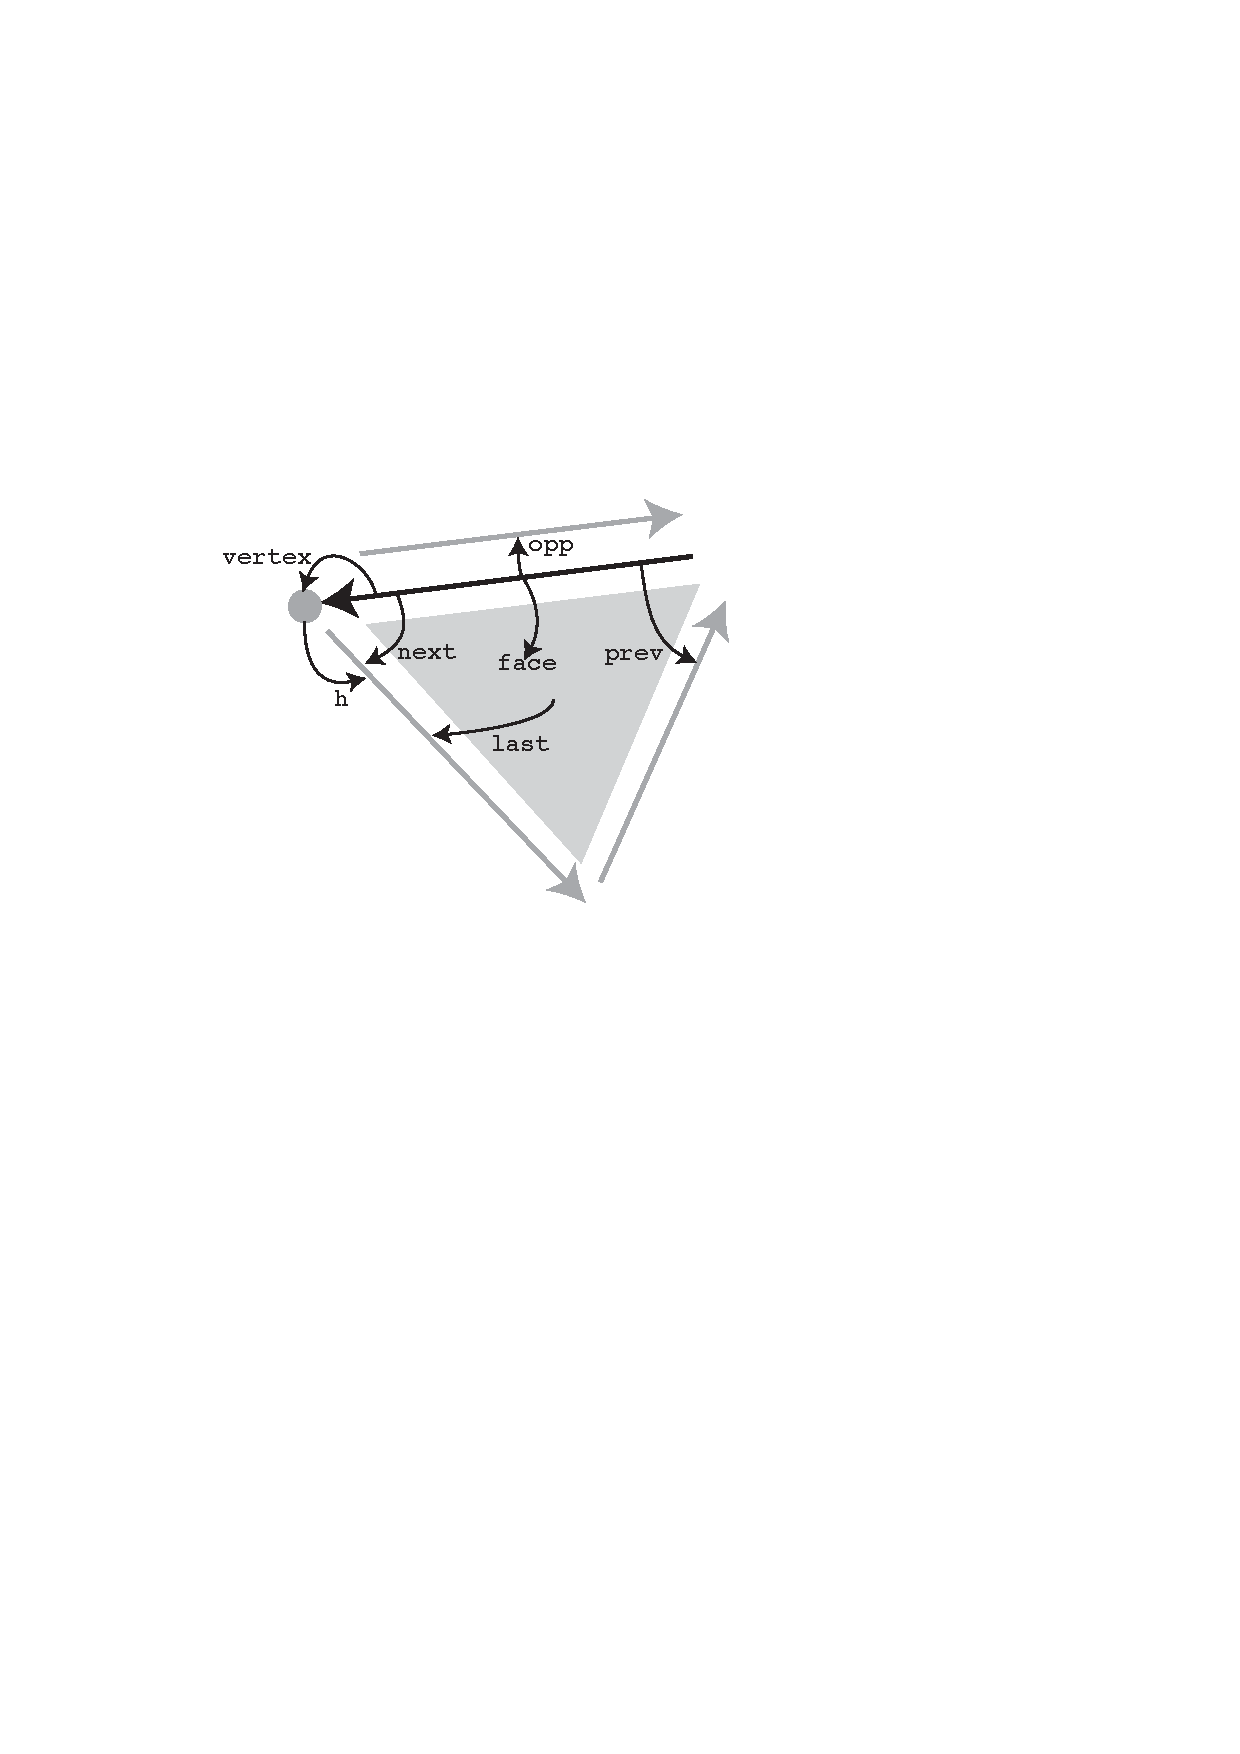
\includegraphics[width=0.5\textwidth]{halfedge-entities.pdf}
\caption{A halfedge and related entities. The halfedge has pointers to the \texttt{next} and previous (\texttt{prev}) halfedges in the counterclockwise loop around its face. It also has a pointer to the opposite (\texttt{opp}) halfedge, which corresponds to the same geometric edge but is part of the loop around the adjacent face. Finally, the halfedge has a pointer to the next \texttt{vertex} in the direction of the halfedge and to its \texttt{face}. A face has a pointer to exactly one halfedge (\texttt{last}) and a vertex has a pointer to one outgoing halfedge (\texttt{h}). The word ``pointer'' is a bit of a misnomer. In GEL we use integer indices instead of memory pointers. }
\label{fig:halfedge}
\end{figure}

The integer indices are not only used to store references from one entity to another. In GEL, we do not directly access entities but use integer IDs to refer to them. For instance to get the position of a vertex, which is stored as a \texttt{Vec3d}, we need
\begin{verbatim}
VertexID vid;
// ... obtain a vertex ID
vec3d p = m.pos(vid);
\end{verbatim}
Note that m.pos(vid) returns a reference to the vertex identified by vid, so we can also assign the vertex position simply using 
\begin{verbatim}
m.pos(vid) = p;
\end{verbatim}
\texttt{VertexID}, \texttt{FaceID}, and \texttt{HalfEdgeID} are simply indices which we use to refer to entities in the mesh. These types are used to communicate with the \texttt{Manifold} class. For instance to get the position of a vertex, but many other functions -- both inside and outside the \texttt{Manifold} class take one of the ID types as argument. For instance,
\begin{verbatim}
VertexID Manifold::split_edge(HalfEdgeID h);
\end{verbatim}
splits an edge and returns a \texttt{VertexID} for the introduced vertex. For functions outside the class, we need to also give the \texttt{Manifold} as an argument since an ID does not tell the function which mesh we are referring to. For example
\begin{verbatim}
bool boundary(const Manifold& m, HalfEdgeID h);
\end{verbatim}
returns true if the halfedge identified by \texttt{h} is a boundary edge in \texttt{m}.

A very frequent operation is that we need to iterate over all the vertices in a mesh. This is done as follows:
\begin{verbatim}
for(VertexID v : m.vertices())
{
   Vec3d p = m.pos(v);
   // Do something with the position
}
\end{verbatim}
Since we also have ID types for faces and half edges, similar code could have been used to iterate over these entities. As a note: there are also specific iterator classes (e.g. \texttt{VertexIDIterator}) which can be used to iterate with old fashioned for loops. However, the syntax is far more cumbersome, so we suggest you stick with the range based for loops as  shown above.
\subsection{Walker}
To loop over all vertices is one way of traversing the mesh. It ensures that we visit all vertices, but it does not relate to the connectivity of the mesh. 
To traverse the mesh in a way that respects connectivity, we use the \texttt{Walker} class. A \texttt{Walker} always points to a specific halfedge, but unlike a \texttt{HalfEdgeID}, it can be used to move from edge to edge. For instance, to compute the centroid for a given face, we can use the following code:
\begin{verbatim}
Vec3d p(0);
FaceID f = m.faces();
Walker w = m.walker(f);
for(; !w.full_circle(); w = w.next())
  p += m.pos(w.vertex()); 
p /= w.no_steps();
\end{verbatim}
The code above computes the centroid for the first face in the mesh. It does so by jumping from edge to edge until it has come full circle. For each jump, we add the vertex pointed to by the halfedge to \texttt{p}. The benefit of the \texttt{Walker} is that it allows us to move from a halfedge to all connected halfedges. The simple traversal functions are \texttt{next}, \texttt{prev}, and \texttt{opp}:
\begin{verbatim}
Walker w;
w = w.next(); 
w = w.prev();
w = w.opp();
\end{verbatim}
\texttt{prev} does the same as \texttt{circulate\_face\_cw} and \texttt{next} does the same as \\\texttt{circulate\_face\_ccw}. The longer names are indicative of the geometric operation while \texttt{prev} and \texttt{next} highlight the connection with the data structure.    It is important to note that all of the functions which operate on \texttt{Walker} instances return a new \texttt{Walker} and do not alter the state of the current walker. Thus to walk around a face, we use \texttt{w = w.next()} as opposed to just \texttt{w.next()} in the for loop above. 
That might seem inconvenient but it is more flexible since we can obtain, say, a nearby vertex just by concatenating some traversal functions. For instance \texttt{w.next().opp().next().vertex()} returns an ID to a vertex nearby  -- without changing \texttt{w}. The sequence \texttt{w.next().opp().next()} creates three anonymous walkers. If, on the other hand, the functions used for walking updated the state of  \texttt{w}, we would have needed to first make a named copy of \texttt{w} before updating its state, so that we could get back to the original state.

\texttt{Walker} can be used to circulate around both faces and vertices. Below, we use vertex circulation to compute the average of the neighbors of a vertex
\begin{verbatim}
Vec3d p(0);
VertexID v = m.vertices();
Walker w = m.walker(v)
for(;!w.full_circle(); w = w.circulate_vertex_ccw()){
  p += m.pos(w.vertex()); 
p /= w.no_steps();
\end{verbatim}

Again, the \texttt{full\_circle()} function tests whether the walker has returned to the original halfedge whence it was created. We can also call  \texttt{no\_steps() } which returns the number of steps taken. In this regard, a step of vertex circulation is considered atomic - even though \texttt{w.circulate\_vertex\_ccw()} is the same as  \texttt{w.prev().opp()}.

From a walker we can easily obtain any of the mesh entities that the halfedge it refers to are incident upon. For instance \texttt{vertex()} returns the \texttt{VertexID} of the vertex which the halfedge points to, \texttt{face()} gives us the \texttt{FaceID} of the incident face and \texttt{halfedge()} simply returns the \texttt{HalfEdgeID}. There is one more option for circulation. The following code does precisely the same as the code above, i.e. it computes the average of the neighboring vertices.
\begin{verbatim}
Vec3d p(0);
int n = circulate_vertex_ccw(m, v, 
          [&](VertexID v){ p += m.pos(v); });
return p / n;
\end{verbatim}
Here the function \texttt{circulate\_vertex\_ccw} takes three arguments. The \texttt{Manifold}, \texttt{m}, and the vertex, \texttt{v}, around which we circulate, and, finally, a function that accepts a \texttt{VertexID}. This function gets called for every vertex adjacent to \texttt{v}. In this example, the function is given as a so called \textit{lambda} function. This allows us to write things compactly and to have the body of the function where it is needed. We could also have passed a function which accepts a \texttt{FaceID} or a \texttt{HalfEdgeID} or a \texttt{Walker}. Thus, we can visit incident faces and edges during circulation if that is what we need, and if we need go get some entity other than adjacent vertices, edges, or faces, we can use the \texttt{Walker} option which is the most generic.

To summarize there are three datatypes that we use to refer to mesh entitites.
\begin{itemize}
\item IDs \texttt{VertexID}, \texttt{HalfEdgeID}, and \texttt{FaceID} are simply indices. These types are what we use when calling functions that take arguments which refer to mesh entities. 
\item ID iterators \texttt{VertexIDIterator}, \texttt{HalfEdgeIDIterator}, and\\ \texttt{FaceIDIterator} as their names imply can be used to iterate over the entities of a mesh. As such they reflect how the mesh is stored in memory. Dereferencing an ID iterator will give an ID. 
\item \texttt{Walker} is used to walk from halfedge to halfedge on the mesh. It utilizes the references stored in halfedges to other halfedges in order to facilitate this traversal. Again, we can obtain an ID from a walker.
\end{itemize}
It might seem tiresome that you have to deal with three different methods for referring to mesh entities, but they do very different jobs. The IDs are simply indices (wrapped in a class) referring to mesh elements. The iterators combine this indices with a reference to the actual data structures. The walker contains functions that allow us to move from halfedge to halfedge and additionally keeps track of the starting point and number of steps taken.

We could have combined two or all three of these concepts, but would have led to rather bloated datatypes.

\subsection{Attributes}
Given a \texttt{VertexID},  \texttt{v}, and a \texttt{Manifold}, \texttt{m}, we can obtain the geometric position of the vertex with the method call \texttt{m.pos(v)}. If is fairly important to note that a reference to the position is returned. Thus, we can assign the position of a vertex:
\begin{verbatim}
Vec3d p;
VertexID v;
// ...
m.pos(v) = p;
\end{verbatim}

Geometric position is in fact the only attribute that is stored for a vertex. That might seem strange since we would very often like to associate any number of attributes with mesh entities. For instance, we might need to associate normals, colors, curvature tensors, counters, etc. with vertices, faces, or even edges.

Unfortunately, what precise attributes we need depends greatly on the precise application. To resolve this issue, we have introduces three attribute vector class templates which allow the user to create his own attribute vectors:
\begin{verbatim}
VertexAttributeVector<T>   vertex_attrib_vector; 
FaceAttributeVector<T>     face_ttrib_vector;
HalfEdgeAttributeVector<T> halfedge_attrib_vector;
\end{verbatim}
where \texttt{T} is a typename. Attribute vectors are indexed with indices. Thus, a
\texttt{VertexAttributeVector} is indexed with a \texttt{VertexID} and likewise for the other types. To give a simple example of how this is used consider smoothing a mesh. The simplest way of smoothing is to replace the vertex with the average of its neighbors. However, if we copy the average value back before the average value for some neighbor has been computed, then we clearly use one average to compute another average and thereby introduce an unfortunate dependence on the ordering of the vertices. Consequently, we need to first compute all of the averages and then update the original vertices. The code looks as follows:
\begin{verbatim}
void smooth(Manifold& m, float t)
{
  VertexAttributeVector<Vec3f> pos(m.total_vertices());
  for(VertexID v : m.vertices())
  { 
    if(!boundary(m, v))
    {
      Vec3f avg_pos(0);
      Walker w = m.walker(v)
      for(; !w.full_circle(); w = w.circulate_vertex_cw())
        avg_pos += m.pos(w.vertex());
      pos[v] =  avg_pos / w.no_steps();
    }
  }
  
  for(VertexID v : m.vertices())
  {
    if(!boundary(m, v))
      m.pos(v) = pos[v];
  }
}
\end{verbatim}

In the smoothing example the \texttt{VertexAttributeVector} containing the new positions is initialized to a size equal to the actual number of vertices. That is not strictly necessary since the attribute vectors automatically resize if the index stored in the ID is out of bounds. Thus, we never explicitly need to increase the size of an attribute vector. What if there are suddenly fewer vertices? In that case, we can clean up the attribute vector. However, we also need to clean up the manifold. The procedure looks as follows:
\begin{verbatim}
VertexAttributeVector<T> vertex_attrib_vector; 
Manifold m;
// ....

IDRemap remap;
m.cleanup(remap);
vertex_attrib_vector.cleanup(remap);
\end{verbatim}
Calling \texttt{cleanup} on the \texttt{Manifold} removes unused mesh entities, resizes, and resize the vectors containing these entities. When we subsequently call cleanup on the attribute vector, the same reorganization is carried out on the attribute vector keeping it in sync. Strictly speaking cleanup is rarely needed, but it removes unused memory which can be a performance advantage.

\subsection{Extended Example: Edge Flipping}
The following example demonstrates how to create a \texttt{Manifold} and add polygons (in this case triangles) and finally how to flip edges of a manifold. First, let us define some vertices
\begin{verbatim}
  vector<Vec3f> vertices(3);
  vertices[0] = p1;
  vertices[1] = p2;
  vertices[2] = p3;
\end{verbatim}
and then a vector of faces. The faces vector contains the number of vertices of each face in the mesh we want tor produce. Initially, we want to make a mesh with just one single triangle, so we produce a vector of one element and set that element to 3.
\begin{verbatim}
vector<int> faces(1);
faces[0] = 3;
\end{verbatim}
Next, we need the index vector. This vector is a long list of indices to vertices. For each face, we store the indices to its vertices in this vector. Since we just have a triangle, we store three vertices in the vector.
\begin{verbatim}
vector<int> indices(3);
indices[0]=0;
indices[1]=1;
indices[2]=2;
\end{verbatim}
So, if we had had two triangles, we would have stored six indices. Finally, we call \texttt{build} with the indexed face set data, we have compiled. 
\begin{verbatim}
m.build(3, reinterpret_cast<float*>(&vertices[0]),1,
   &faces[0], &indices[0]);
\end{verbatim}
The result of the above is a mesh with a single triangle.
Next, we try to split an edge. We grab the first halfedge and split it: Now we have two triangles. Splitting the halfedge changes the containing triangle to a quadrilateral, and we call triangulate to divide it into two triangls again.
\begin{verbatim}
HalfEdgeID h = m.halfedge();
m.split_edge(h); 
triangulate_face_by_edge_split(m, m.walker(h).face());
\end{verbatim}
Now, we obtain an iterator to the first of our (two) triangles.
\begin{verbatim}
FaceID f1 = m.faces();
\end{verbatim}
We create a vertex, \texttt{v}, at centre of \texttt{f1} and insert it in that face:
\begin{verbatim}
m.split_face_by_vertex(f1);
\end{verbatim}
The code below, marks one of a pair of halfedges (with the value 1).
\begin{verbatim}
HalfEdgeAttributeVector<int> touched;

// ....

for(HalfEdgeID h : m.halfedges())
{
  if(m.walker(h).opp().halfedge() < h)
    touched[h] =0;
  else
    touched[h] =1;
}
\end{verbatim}
Next, we set the \texttt{flipper} variable to point to the first of these halfedges:
\begin{verbatim}
flipper = m.halfedges_begin();
\end{verbatim}
The long piece of code below examines a halfedge pointed to by \texttt{flipper}, and if it is not a boundary halfedge it tries to flip it. Then it increments the \texttt{flipper} variable until it lands on a halfedge marked with 1. If \texttt{flipper} reaches the end of the list of halfedges, we start over.
\begin{verbatim}
  if(!boundary(m, *flipper)) 
      if(precond_flip_edge(m,*flipper))
                m.flip_edge(*flipper);
  do
    {
      ++flipper;
      if(flipper==m.halfedges_end())
        {
          flipper = m.halfedges_begin();
          break;
        }
    }
  while(touched[*flipper] == 0);
\end{verbatim}
This example may not serve much of a purpose but illustrates how we can iterate over all edges and flip them. From this example, we are fairly close to Delaunay triangulation.

\subsection{HMesh tools}

The HMesh directory contains not only the basic data structure and functionality for traversing a mesh. There are also tools for mesh optimization through energy minimization, several algorithms for mesh smoothing, a number of tools for cleaning meshes as well as tools for simplifying meshes.
%
%
\section{GLGraphics}
%
%
\texttt{GLGraphics} contains a set of tools needed for visualization of geometrical objects. In particular, this namespace contains mesh rendering facilities, and in the following, a very simple example is given. This section is basically a walk through of the simplest GEL program that draws a mesh. Apart from GEL, we also use OpenGL and that requires a toolkit for connecting with the window system. With GEL programs, one generally uses GLUT, and this example is not an exception.

For starters, we need to include some files mostly from \texttt{GLGraphics} but also the header file for the mesh load function of \texttt{HMesh} and the \texttt{GLEW} header. Why incude \texttt{glew.h} rather than just \texttt{gl.h}? Well, \texttt{HMesh/draw.h} contains some draw functions which rely on shaders, and since \texttt{gl.h} is normally not up to date, it makes sense to use \texttt{glew.h} instead of \texttt{gl.h} even though it inflicts a dependency. We include \texttt{GLGraphics/gel\_glut.h} rather than the normal \texttt{glut.h}. That is because the GEL version works the same on Windows, OSX, Linux and probably other platforms.

We also open the namespaces we will need and declare two globals: The view controller \texttt{view\_ctrl} and the mesh \texttt{mani}. The view controller class is rather complex. It more or less insulates you from having to deal directly with the projections and transformations of OpenGL: It sets up a perspective projection and also the modelview transformation needed to view the object. From a user interface perspective, it defines a virtual trackball which allows you to rotate the object.
\begin{verbatim}
#include <GL/glew.h>
#include <GLGraphics/gel_glut.h>
#include <GLGraphics/draw.h>
#include <GLGraphics/GLViewController.h>
#include <HMesh/load.h>

using namespace std;
using namespace HMesh;
using namespace CGLA;
using namespace GLGraphics;

GLViewController* view_ctrl;
Manifold mani;
\end{verbatim}

Below is the display function which is called from the GLUT event loop whenever an event that requires redrawing is received. All drawing takes place inside this function. In this case, it is simple since all we need to do is clear the screen (and depth buffer), set up a new modelview transformation with the view controller and then call the draw function followed by a swap of buffers.

The draw function sends the polygons to the graphics card. It is very inefficient and uses the fixed function pipeline. At a minimum one should draw the polygons to a display list, but for a simple example, this works. The buffer swap is because we use double buffering; in other words, we draw to the back buffer.
\begin{verbatim}
void display() {
    glClear(GL_COLOR_BUFFER_BIT | GL_DEPTH_BUFFER_BIT);
    view_ctrl->set_gl_modelview();
    draw(mani);
    glutSwapBuffers();
}

\end{verbatim}
The mouse callback below is called when a mouse event has occurred. This is where user input  for the virtual trackball is registered. We check whether a mouse is pressed or released. If it is pressed, we detect which button and then ``grab'' the virtual trackball in order to rotate, zoom, or pan depending on which button is pressed. If the button is released, we inform the view controller of this.
\begin{verbatim}
void mouse(int button, int state, int x, int y)  {
    Vec2i pos(x,y);
    if (state==GLUT_DOWN) 
    {
        if (button==GLUT_LEFT_BUTTON) 
            view_ctrl->grab_ball(ROTATE_ACTION,pos);
        else if (button==GLUT_MIDDLE_BUTTON) 
            view_ctrl->grab_ball(ZOOM_ACTION,pos);
        else if (button==GLUT_RIGHT_BUTTON) 
            view_ctrl->grab_ball(PAN_ACTION,pos);
    }
    else if (state==GLUT_UP)
        view_ctrl->release_ball();
}
\end{verbatim}
If the mouse moves with a button depressed, we register motion in the function below. The new mouse position is sent to the view controller
which then, e.g., rotates the trackball accordingly. Note that this function ends by posting a redisplay event, i.e. informs GLUT that display should be called at the earliest convenience.
\begin{verbatim}
void motion(int x, int y) {
    Vec2i pos(x,y);
    view_ctrl->roll_ball(Vec2i(x,y));
    glutPostRedisplay();
}
\end{verbatim}

Finally, in the main function, we first load the mesh and then setup glut. This mostly involves defining the callback function just described. We set up the view controller passing it window dimensions and the size and position of the bounding sphere of the object just loaded. Finally, we do some minimal OpenGL set up: Essentially clearing the depth buffer and enabling lights. Finally, we pass control to the GLUT event loop.
\begin{verbatim}
int main(int argc, char** argv) {
    string file = "bunny-little.x3d";
    load(file, mani);

    glutInitDisplayMode(GLUT_RGBA|GLUT_DOUBLE|GLUT_DEPTH);
    glutInitWindowSize(800, 800);
    glutInit(&argc, argv);
    glutCreateWindow("GEL Example Program");
    glutDisplayFunc(display);
    glutMouseFunc(mouse);
    glutMotionFunc(motion);
    
    Vec3f bsphere_center(0,0,0);   
    float bsphere_radius = 3;
    mani.get_bsphere(bsphere_center,bsphere_radius);
    view_ctrl = new GLViewController(800,800, 
        bsphere_center,bsphere_radius*2);
    
    glClearColor(0.0f, 0.0f, .5f, 0.f);
    glEnable(GL_DEPTH_TEST);
    glEnable(GL_LIGHTING);
    glEnable(GL_LIGHT0);
    
    glutMainLoop();
}
\end{verbatim}
Note that the mesh can be either an X3D, OBJ, PLY, or OFF files. However, only the geometry is loaded not the textures. In the case of OBJ files, we also convert all polygons to triangles, because the TriMesh loader (see the geometry class) is in fact used.

Apart from the drawing functions and the viewcontroller, GLGraphics also contains  other useful pieces: A few functions which greatly simplify shader loading and SOIL. SOIL is a small library for loading images. It is designed for OpenGL and makes it easy to e.g. save screen shots or load an image for use as a texture. While the need for image loading is fairly obvious, it might be more difficult to see the need for shader loading functions. However, it \textit{is} a little tricky to make shader programs in C++ using GLSL but the problems are almost all silly little things. For instance, how do you robustly read from a text file? How do you compile a shader and check for errors? In OpenGL What is the difference between a GLSL program and a shader anyway?

The short answer to the last question is this: A "shader" can be either a vertex shader, a geometry shader (in OpenGL 2.0) or a fragment shader. A "program" is a linked combination of these three types of shaders. Note that you don't have to have a geometry shader.

These functions attempt to obviate the need for an answer to the first two questions by providing an API for loading and compiling shaders and checking for errors. However, I don't include functions for creating the program, attaching shaders and linking. Why not? Because the need for flexibility means that the API would be just as complex as just using the OpenGL functions directly! However, loading shaders and checking for errors in compiled shaders is different. It makes sense to wrap that. It also makes sense to wrap the error checking for programs that are linked, so there is a function for that too.

Since shader loading and error check sandwhich the two calls needed for compilation, the most important function in this API, \texttt{create\_glsl\_shader}, loads a shader, compiles it, checks for errors and returns the shader handle. There is also a version which creates a shader from a string.

There is some code below to illustrate usage.  
\begin{verbatim}
GLuint vs = create_glsl_shader(GL_VERTEX_SHADER, 
  shader_path, "tri.vert");
GLuint gs = create_glsl_shader(GL_GEOMETRY_SHADER_EXT, 
  shader_path, "tri.geom");
GLuint fs = create_glsl_shader(GL_FRAGMENT_SHADER, 
  shader_path, "tri.frag");

prog_P0 = glCreateProgram();

if(vs) glAttachShader(prog_P0, vs);
if(gs) glAttachShader(prog_P0, gs);
if(fs) glAttachShader(prog_P0, fs);

// Specify input and output for the geometry shader.
// Note that this must be done before linking the program.
glProgramParameteriEXT(prog_P0,GL_GEOMETRY_INPUT_TYPE_EXT,
  GL_TRIANGLES);
glProgramParameteriEXT(prog_P0,GL_GEOMETRY_VERTICES_OUT_EXT,3);
glProgramParameteriEXT(prog_P0,GL_GEOMETRY_OUTPUT_TYPE_EXT,
  GL_TRIANGLE_STRIP);

// Link the program object and print out the info log
glLinkProgram(prog_P0);
print_glsl_program_log(prog_P0);

// Install program object as part of current state
glUseProgram(prog_P0);

// Set the value of a uniform
glUniform2f(glGetUniformLocation(prog_P0,"WIN_SCALE"), 
  win_size_x/2.0, win_size_y/2.0);
\end{verbatim}
%
%
\section{Geometry}
%
%
The Geometry namespace contains many different classes and functions. Roughly, we can divide the contents into
\begin{itemize}
\item Spatial data structures such as kd tress, bounding box hierarchies, and BSP trees.
\item A Triangle mesh data structure called TriMesh. TriMesh is different from HMesh in that it only contains triangles. It is much more an API for real time rendering which also facilitates material properties and not just geometry.
\item Classes and functions for dealing with volume data. HGrid and RGrid are, respectively, a class for hierarchically stored voxel grids (sparse grids) and regular grids. There is a number of functions for traversing voxel grids systematically and along rays.
\item Surprisingly, you will also find my C++ port of Jules Bloomenthals isosurface polygonizer and an implementation of Luiz Velho's parametric surface tiler in this namespace.
\end{itemize}
One of the most frequently used tools in Geometry is the kD tree class which merits an example. In the code below, we create a kD tree which had \texttt{Vec3f}s as keys and integers as data. Note that since the kD tree is a template, we could use any other type as both key and data, however, only CGLA vectors have been tested as key types, but there are no restrictions on data types.
\begin{verbatim}
    KDTree<Vec3f,int> tree;
    for(int i=0;i<N;++i)
        {
            Vec3f p0;
            make_ran_point(p0);
            tree.insert(p0, i);
        }
    tree.build();
\end{verbatim}
Note also, that before we use the tree it needs to be built. This is because the internal representation is a balanced binary heap which it is easier to build at the end rather than maintain during insertion of new points. To look for the points near a given point, we can call
\begin{verbatim}
    Vec3f p0;
    // ...
    std::vector<Vec3f> keys;
    std::vector<int> vals;
    float radius = 1.95f;
    int N = tree.in_sphere(p0, radius , keys, vals);
\end{verbatim}
This will find all points in a radius of 1.95 units from \texttt{p0}. The keys and values are stored in \texttt{keys} and \texttt{vals} when the functions returns. The return value of the function is the number of points found within the radius. 

Sometimes, we simply want the point closest to a given point \texttt{p0} which is done using \texttt{tree.closest\_point(p0, d, pos, x)} where the two first arguments indicate the point and the maximum search radius. The two last arguments are set to the key and data of the point found to be closest to \texttt{p0}. The function returns true if a closest point was found.
%
%
\section{Util}
%
%
The Util namespace contains a rather mixed bag of utilities many of which are quite useful and very diverse. 
\begin{trivlist}
\item The XML parser for instance is written from scratch and the basis for our X3D loader although it will load any XML file. 
\item \texttt{Grid2D} is often useful when we want to deal with e.g. simulation on a 2D grid. 
\item The \texttt{Timer} class is nearly indispensable when we need to time something, and it is very easy to use. 
\item \texttt{ArgExtracter} is a class for getting the command line arguments to a program. 
\item There is more - for instance a resource manager template, some string utility templates and a hash table implementation.
\end{trivlist}
Arguably, it would be more pretty if these pieces had been more thematically linked, but many are used a lot, and it seemed reasonable to have somewhere to stick various functions and classes that did not naturally belong elsewhere.
%
%
\section{Authors}  
%
%
\begin{trivlist}
\item Andreas B{\ae}rentzen created the library and has written most of the code not contributed by the people below.
\item Jeppe Revall Frisvad has contributed greatly to the CGLA part of GEL and elsewhere.
\item Christian Thode Larsen rewrote the classes in HMesh. They are much nicer for it.
\item Anders Wang Kristensen has been a great help in the process of reworking HMesh and also contributed some code for an OpenGL console.
\item Henrik Aan{\ae}s provided the original LinAlg package, which is a set of simple but very useful Lapack bindings. However, these were later removed. GEL and PyGEL do not require a numerics library, and we now use Eigen in applications that use GEL.
\item Rasmus Paulsen, Bjarke Jakobsen, Marek Misztal helped with structure and compilation on various platforms with testing and ideas.
\end{trivlist}
%
%
\section{License}  
%
%
\begin{trivlist}
\item
You are allowed to use GEL for academic or commercial purposes. In particular, you are welcome to give GEL to students as a basis for academic work or to use it in your own applications.
\item
Regarding the use of GEL in other libraries. GEL does exist in slightly different versions, since we have created pared down packages for various courses. We would like to retain the prerogative of repackaging. If you would like to use GEL in its entirety in another library  that is fine, but we do not allow you not to take bits and pieces and put them into a different library.
\item
If you use GEL, we would be grateful for due credit.
\item
Finally, we follow the MIT license as regards warranty:
\item
THE SOFTWARE IS PROVIDED "AS IS", WITHOUT WARRANTY OF ANY KIND, EXPRESS OR IMPLIED, INCLUDING BUT NOT LIMITED TO THE WARRANTIES OF MERCHANTABILITY, FITNESS FOR A PARTICULAR PURPOSE AND NONINFRINGEMENT. IN NO EVENT SHALL THE AUTHORS OR COPYRIGHT HOLDERS BE LIABLE FOR ANY CLAIM, DAMAGES OR OTHER LIABILITY, WHETHER IN AN ACTION OF CONTRACT, TORT OR OTHERWISE, ARISING FROM, OUT OF OR IN CONNECTION WITH THE SOFTWARE OR THE USE OR OTHER DEALINGS IN THE SOFTWARE.
\item
If anything is unclear, please send an email to jab@imm.dtu.dk. 
\end{trivlist}
%
%
\section{Open Source Code used in GEL}  
%
%
Source code from other projects have been incorporated in GEL.
\begin{trivlist}
\item From Graphics Gems, two functions for inverting matrices and Jules Bloomenthal's polygonizer which I reworked from C to C++. This is allowed according to the license.
\item rply by Diego Nehab, Princeton University, and the Simple OpenGL Image Loader by Jonathan Dummer.  These are MIT licensed and our use is congruent with that license.
\item The OpenGL Extension Wrangler Library is also included and appears to have a license identical to the MIT license.	 As mentioned, our use is congruent with that license.
\end{trivlist}
The incorporated code amounts to only a small fraction of the GEL source code.
\end{document}
